\section{Patent, copyright and trademark}
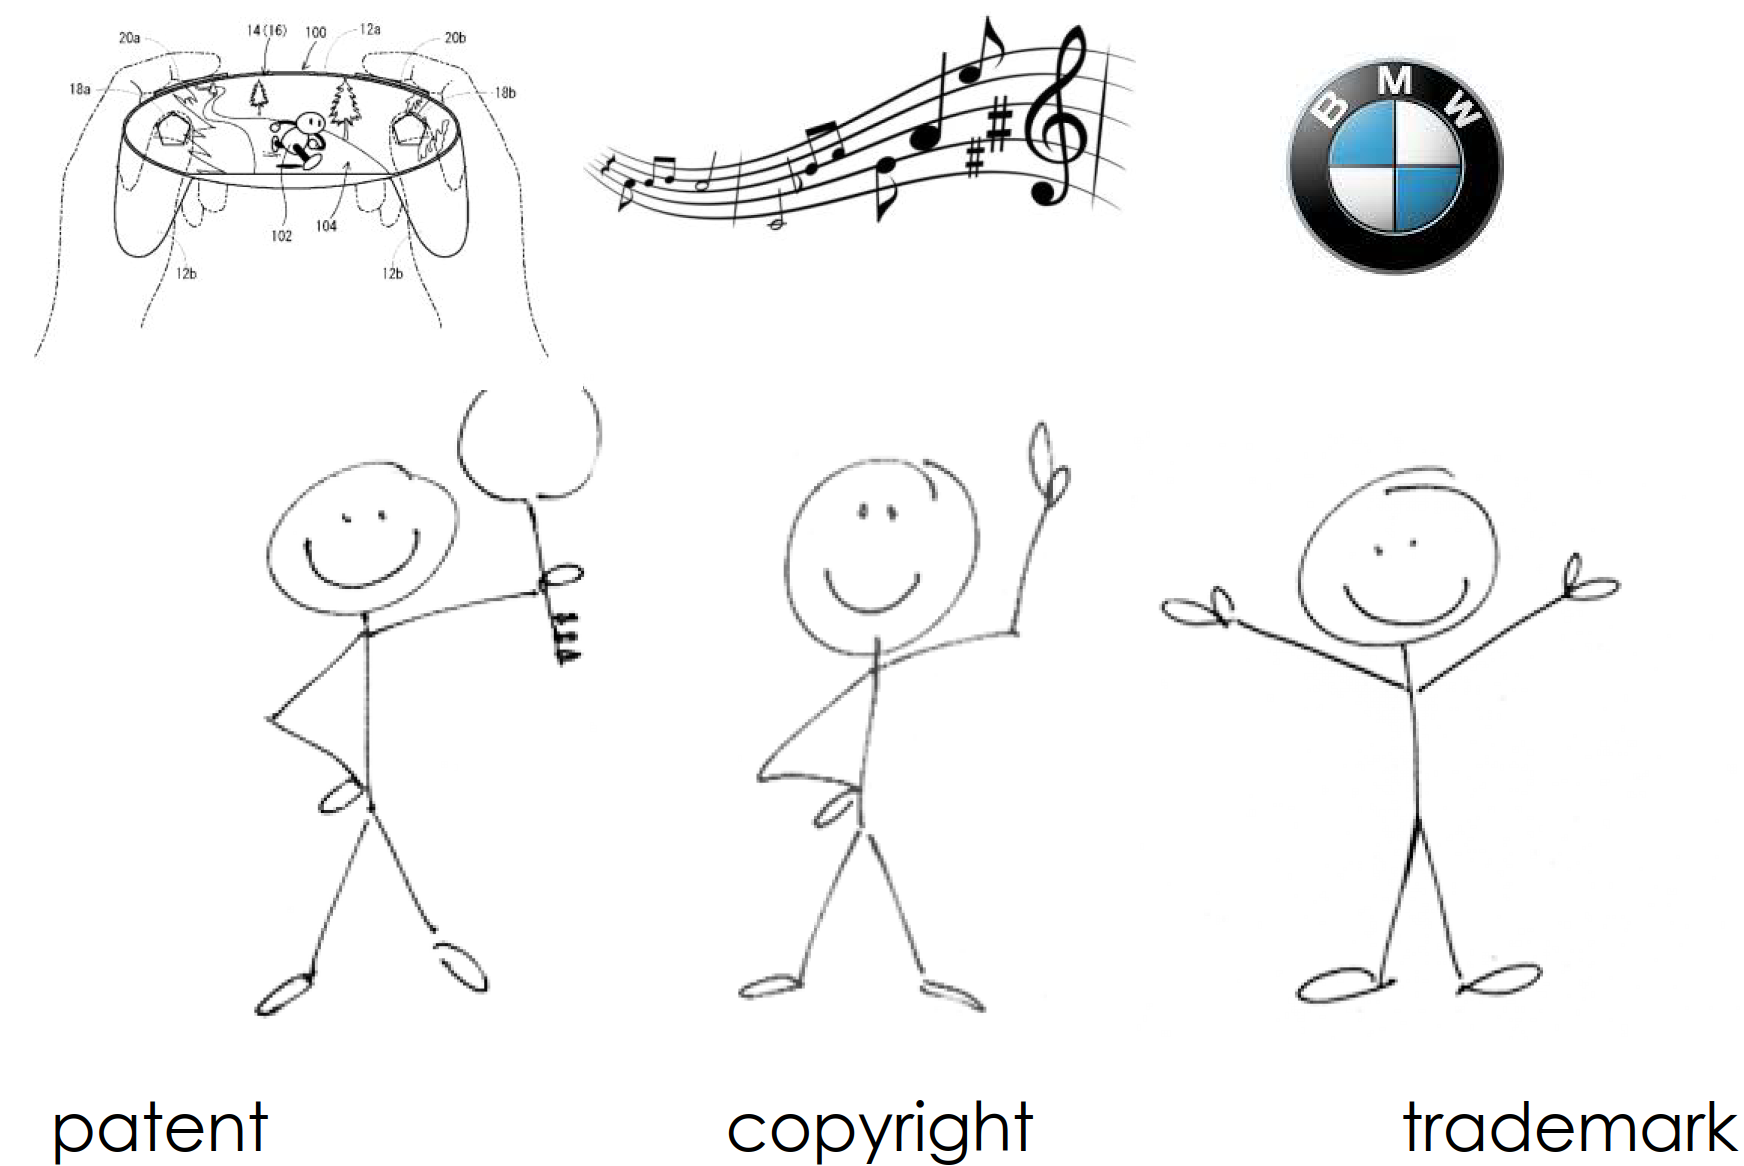
\includegraphics[width=1\linewidth]{images/patent_copyright_and_trademark}
Protection is limited to the form expressing an idea. Ideas as such or a mere concept are not protected. Ideas need to flow freely!

\subsection{Copyright}
\subsubsection{Purpose of copyright law}
Through their works and performances, creative artists contribute to our country's cultural diversity . However they also want to earn something with their works and performances.
\begin{compactitem}
	\item The copyright law guarantees them financial remuneration for the utilization of their works. 
	\item The copyright law protects artists intellectual property in that they are able to defend themselves against misappropriation of their work.
	\item Copyright is a tool with which to earn something from cultural creativity. It is thus a part of our liberal economic and social order which safeguards property (including intellectual property). 
\end{compactitem}

\subsubsection{Definition of a "work"}
\begin{compactitem}
	\item Texts
	\item Music
	\item Photography
	\item Works of fine art
	\item Works with scientific content
	\item Architecture
	\item Visual and audiovisual works
	\item Choreographies and pantomimes
	\item Computer programs
\end{compactitem}

\subsubsection{Prerequisites for legal protection of a work}
\textbf{Prerequisites for legal protection:}
\begin{compactitem}
	\item Intellectual creation
	\item Individual character
	\item Perceptability / expression of an idea
	\item Irrespective of any value or purpose
	\item Work created by humans
\end{compactitem}
\textbf{“Statistical Uniqueness”, abstract criteria:}
\begin{compactitem}
	\item Characteristic features
	\item No one else would have created the work that way
	\item Sufficiently creative step beyond sheer otherness
	\item Work is something unique and special
\end{compactitem}
\textbf{Individual character:} \\
Analysis of concrete criteria for each category of work, eg photography
\begin{compactitem}
	\item Selection of object, image section and time of triggering
	\item Design of the image components
	\item Distribution of light and shadow
	\item Use of specific lenses or filters
	\item processing of the negative
\end{compactitem}

\subsubsection{Work and work copy}
Work: Intangible good / intellectual property (eg. Firefox)\\
Work copy: materialized work, ie physically existent, often (but not necessarily) physical expression of the work (eg. Firefox installed on a computer)

\subsubsection{Second hand work}
\begin{compactitem}
	\item Creation using pre-existing works
	\item Independent protection of these works, if protection requirements fulfilled
	\item Protection of the existing works is reserved
	\item Creative change of a pre-existing work
	\item Individual character and thus independent protection of processing. But: individual character of the existing work still recognizable
	\item Example: Translation, filming, staging
\end{compactitem}

\subsubsection{What is copyright?}
\begin{compactitem}
	\item Author of a copyrighted work is always the natural person who created the work (“creator principle”). Copyright law is an absolute right and thus excludes every other person.
	\item Copyrights can be transferred from the original author to another person/legal entity who then becomes the right holder.
\end{compactitem}

\subsubsection{Moral rights}
\begin{compactitem}
	\item Recognition of authorship
	\item First publication
	\item Integrity of the work
\end{compactitem}
Moral rights vest in the author and cannot be transferred/licensed.

\subsubsection{Authorship}
\textbf{Joint Authors:} \\
When multiple people work together pursuant to a common concept to create a work together. The joint authors can only decide jointly on what happens with the work. Conclude a contract! \\
\textbf{Copyright and Employment:} 
\begin{compactitem}
	\item General rule: the author is right holder upon creation. The employer is not entitled unless employee transfers the copyrights within individual employment contracts.
	\item Exception: the law assumes that copyright in a computer program vests in the employer if an employee creates the computer program during working hours as part of his or her job.
\end{compactitem}

\subsubsection{Duration of copyright}
A work is protected under copyright as soon as it is created . It is not necessary to file for protection or to “deposit” the work. In Switzerland there is no register.\\
\textbf{Not required:}
\begin{compactitem}
	\item Having the work recorded on a carrier (printed book, pressed CD)
	\item Publication of the work
	\item The explicit will to create work
	\item Ability to act: authors can, for example, also under-assisted or hypnotized persons
\end{compactitem}
\textbf{Formalities:} \\
It is also not necessary to refer to the copyright in the work. Notations such as “copyright“, “all rights reserved“ or “©” have no influence on protection in Switzerland. In other countries the notification can be important for copyright protection. \\
\textbf{Duration:}
In Switzerland copyright protection expires 70 years after the death of the author. Exception: the protection for computer programs ends 50 years after the death of the author.

\subsubsection{Limitations of copyright}
Whoever publishes, reproduces, performs, broadcasts or otherwise disseminates a work requires the author’s consent. However: Private use is not subject to license fees. But that does not apply to computer programs: Permission from the rights holder must be obtained for each use!

\subsubsection{Related rights}
The Copyright Act also regulates related rights (or neighboring rights).
\begin{compactitem}
	\item the rights of performing artists (musicians, actors) to their performances;
	\item the rights of producers of phonograms and videograms to their products (CD, DVD);
	\item the rights of broadcasters to their radio and television broadcasts.
\end{compactitem}
Related rights protection expires 50 years after the performer’s performance, the publication of the phonogram or videogram (or the production of it, in the case that it is not published) or the emission of the broadcast. The rights of a performing artist to be named as performer ends upon his or her death, or 50 years after the performance, at the earliest.

\subsubsection{Legal protection}
\textbf{Civil procedures:} \\
Civil proceedings involve copyright claims between private persons/private legal entities.
The author/right holder can request from the civil court
\begin{compactitem}
	\item a declaratory judgment (have a right established);
	\item have an infringement banned/remedied;
	\item have property confiscated;
	\item have an order published.
\end{compactitem}
\textbf{Criminal procedures:} \\
Criminal procedures may be initiated by the right holder within 3 months after becoming aware of an infringement or the authorities. \\
Fines or imprisonment of up to 1 year (or 5 years if committed on a commercial basis) for use without the right holder’s consent in particular:
\begin{compactitem}
	\item use of a work within correctly indicating the author
	\item publishing a work
	\item change a work
	\item use for derivative work
	\item copies of works
	\item distributing or making works available
	\item broadcasting
	\item renting out of computer programs
\end{compactitem}

\subsubsection{Collecting Societies}
The Federal Copyright Act is based on the view that the rights accruing to authors are essentially the responsibility of the right holders to assert for themselves. The Federal Copyright Act only envisages collective management by collective rights management organizations in circumstances where mass utilization makes direct management virtually impossible.

\subsubsection{Copyright law and Internet}
\textbf{Use of content:} \\
Downloading, copying, scanning, etc., are types of use of a copyrighted work. \\
The right holder has the right to give permission to any kind of use of his work or to revoke this permission. This permission must be given expressly (verbally or in writing) or implied. \\
When published works are used as sources in the Internet, they must be cited in the way books are cited; otherwise plagiarism is taking place. \\
\textbf{Links:} \\
This first of all facilitates access to the linked page (by clicking directly on the link), and secondly implies to the internet user that the linked pages are associated. This assumption can be wrong. Therefore, rights can in fact be infringed simply through linking, such as those contained in the Federal Act against Unfair Competition (UCA) or the Data
Protection Act (DPA). Therefore, linking should always be agreed upon between the parties.

\subsubsection{Federal copyright act}
The Federal Copyright Act of 1992, is the legal basis for the protection of literary works and works of art. It is currently under revision. It also governs what are known as “neighboring rights”, i.e. the rights of performers, record producers and broadcasting companies. The Federal Copyright Act stipulates the rights and obligations of the five
collective administration societies.

\subsection{Trademark}
A trademark is a protected sign which is used to identify a product or service and to distinguish the products or services of one business from another. Basically, any graphic representations can be used as trademarks under the law:
\begin{compactitem}
	\item words (eg. Victorinox)
	\item combinations of letters (e.g. SBB),
	\item numericals (eg. 501),
	\item graphic images (eg. the Swisscom logo),
	\item three-dimensional forms (eg. the Mercedes star),
	\item slogans (eg. “Cats would buy Whiskas”),
	\item any combination of these elements,
	\item jingles, a series of tones (acoustic trademarks, eg. the Ricola jingle)
\end{compactitem}

\subsubsection{Purpose of trademark law}
Trademarks influence consumer decisions every day. A strong trademark creates an identity, builds trust, distinguishes from competitors, and facilitates communication between producers and consumers.
\begin{compactitem}
	\item \textbf{Exclusive right:} Registering a trademark gives you the exclusive right to use a certain sign for specific goods and services.
	\item \textbf{Monetize:} You may grant someone else the right to use your trademark it through licensing.
	\item \textbf{A trademark offers protection:} As a trademark owner you can prevent others from using an identical or
	similar sign for the same or similar goods and services.
\end{compactitem}

\subsubsection{Meaning of a trademark}
The owner of a trademark work is entitled to the exclusive and sole right in the trademark to determine $\overset{1}{\text{\textbf{what} }}$ $ \overset{2}{\text{\textbf{when} }} \overset{3}{\text{\textbf{how} }}$ $\overset{4}{\text{\textbf{by whom}}}$ may be done with his or her trademark.

\subsubsection{Company name}
It is often wrongly assumed that the name of a business is automatically protected as a trademark. You should register your company name:
\begin{compactitem}
	\item in the commercial register
	\item in the trademark register
	\item with switch.ch to obtain a domain name
\end{compactitem}

\subsubsection{Grounds for refusal of registration}
\begin{compactitem}
	\item Signs which belong to the public domain must remain available to everyone and cannot be registered.
	This includes, for instance, single letters or numbers or abbreviations. A sign may also not be purely descriptive of a characteristic, quality, type or place of production (generic names). Example: «apple» cannot be registered for a type of apple or fruit but it can be registered for a computer!
	\item A trademark may also not be misleading or deceptive regarding	properties such as source or quality. Example: the trademark «GoldArt» cannot be registered for goods which are not made of gold or gilded with gold.
	\item A trademark also may be offensive to moral standards or against the law.
\end{compactitem}

\subsubsection{Colors}
As a rule, individual colors cannot be protected. Exception: colors that have come to be accepted as being distinctive and
have gained the character of a trademark through everyday use (eg. Milka).

\subsubsection{Classes of goods and services}
A trademark is not protected in general but only for those classes of goods and services for which it has been registered. When you register, you must indicate the goods and services for which you wish to register and use your trademark. \\
If you don’t use your trademark for the products (or services) you claimed within five years of registration, you can lose your trademark protection: in a litigation, the other party could claim that you do not use your trademark.

\subsubsection{Duration of trademark protection}
A trademark is protected once it is registered. The term of protection is 10 years. The 10-year term of protection can be renewed multiple times. As there is no time limit, a trademark that is actually in use can be protected indefinitely. Trademark rights are reserved for whoever registers first. A trademark must also actually be used within the five years following its registration. A trademark should remain unpublished before you apply for registration. If not, someone else can register it in their name.

\subsubsection{«Trademark registered»}
It is not compulsory to use the ® sign in Switzerland. Actually, it makes no difference if you use the ® sign or not. Using the ® sign without having actually registered the mark is an offense!

\subsubsection{International trademark protection}
Trademarks are only valid in the country where they are registered. A trademark registered in Switzerland is therefore only protected in Switzerland. If the trademark should also be protected in other countries, then you must register it there too. In most cases, even so-called regional or international registration proceedings merely result in purely national autonomous IP rights.
\begin{compactitem}
	\item \textbf{Applying directly to the country concerned:} Be aware that the legal basis, filing formalities as well as examination and	granting procedures vary from country to country (costs!).
	\item \textbf{The Madrid System:} Under the Madrid System you can extend the trademark protection granted under Swiss law to other contracting states or organisations.
	\item \textbf{EU Community Trademark:} By filing one single trademark application at the Office for Harmonization in
	the Internal Market (OHIM) in Alicante, Spain, you can protect your trademark in the entire EU territory with a community trademark. Under the Madrid System, an extension to protection in the	countries of the European Union can also be applied for.
\end{compactitem}

\subsubsection{Filing a trademark}
Trademarks may be registered without any guarantee, the IGE only verifies certain formalities and prerequisites. The IGE does not verify whether identical or similar IP rights such as trademarks, company or domain names already exist. Potential conflicts with rights of other people are not examined within the registration process! \\
The owner of an earlier trademark may file opposition to a new trademark during the three months following the latter’s publication in which he can claim that there is a danger of confusion with his earlier trademark. \\
\textbf{Rules before registering:}
\begin{compactitem}
	\item Make sure your sign is distinctive!
	\item Search trademark registries
	\item Search commercial register and domain names!
\end{compactitem}

\subsubsection{Opposition or Cancellation}
\begin{compactitem}
	\item \textbf{Opposition proceedings:} With publication on www.swissreg.ch, the three-month opposition period
	begins: owners of prior trademarks that are identical or similar to yours can file opposition to your mark during this period.	If the IGE rejects your within an opposition procedure application, you can file an appeal to the Federal Administrative Court within 30 days.
	\item \textbf{Cancellation proceedings:} For cancellation proceedings on the grounds of non-use, any person is
	allowed to request the cancellation of a trademark registration. The request for cancellation may be made at the earliest five years after expiry of the opposition period or, in the case of opposition proceedings, five years after the conclusion of opposition proceedings. The request for cancellation must be justified, in particular, by credibly
	showing non-use of the disputed trademark.
\end{compactitem}

\subsubsection{Infringements}
Protecting the market position of your trademarks is solely your responsibility.
\begin{compactitem}
	\item \textbf{At the time of registration:} Since the IGE do not officially verify the risk of confusion and thus the possibility	of conflict between trademarks, it is essential for you to monitor the market.
	\item \textbf{Anytime:} If you detect an infringement of your trademark rights, you can initiate civil or criminal proceedings in court.
\end{compactitem}
The right holder of a trademark may prohibit others from using a sign from:
\begin{compactitem}
	\item affixing the sign to goods or their packaging;
	\item offering goods, placing them on the market or stocking them for such	purposes under the sign;
	\item offering or providing services under the sign;
	\item importing, exporting or carrying in transit goods under the sign;
	\item using the sign on business papers, in advertising, or otherwise in the course	of trade.
\end{compactitem}
The following may be sanctioned by imprisonment or a fine:
\begin{compactitem}
	\item appropriates, counterfeits or imitates the trademark of the other person;
	\item places goods on the market or provides services, or offers, imports, exports, carries in transit or advertises such goods or services under the appropriated, counterfeited or imitated trademark.
	\item unlawfully labels goods or services with the trademark of another person in order to mislead and thereby give the impression that the goods or services are original goods or services;
	\item offers or places goods or services on the market as original goods or services, or offers or provides original services that unlawfully bear the trademark of another
\end{compactitem}
Whoever imports counterfeit brand products for their own personal use risks that the goods will be seized by customs.

\subsubsection{Special trademarks}
\textbf{Indication of source:}\\
Indications of source do not differentiate certain goods or services from each other by the manufacturer of the product as trademarks do, but by their geographical origin. They may only be used for products which originate from the indicated geographical area. With signs for services, the service provider must show an adequate association with the claimed geographical indication of source (eg. registered office in the country concerned).\\
\textbf{Collective mark:}\\
A collective mark identifies the products of an association of companies. Regulations specify who may use the trademark.\\
\textbf{Guarantee mark:} \\
A guarantee mark signifies that a product is guaranteed to have certain properties or qualities (e.g. quality characteristics). If the goods or services of a supplier have the guaranteed properties, the latter may use the guarantee mark as long as he or she pays the owner appropriate compensation. To avoid any conflict of interest, the trademark owner is not allowed to use the trademark himself nor have a commercial relationship with those using the trademark.

\subsection{Design}
\subsubsection{Definition design} 
In the legal sense, design is understood to be the exterior form of a product or parts of it. It can be either two-dimensional (a pattern) or three-dimensional. Its form is characterised by the arrangement of lines, contours, colours and surfaces or by the material used.

\subsubsection{Protection of designs}
Design appeals to our senses, evokes feelings, creates identity and distinguishes itself. This is why design has become one of the most crucial market factors and why counterfeiting is subsequently a frequent occurrence in this field. Owners of a design right can prevent others from using products with the same or a similar design.

\subsubsection{Filing a design}
\textbf{Criteria:} 
\begin{compactitem}
	\item The design is new , meaning no other identical or similar design has been	published before application;
	\item The design is sufficiently different from existing designs in major characteristics.
\end{compactitem}
The IGE does not examine a design for newness or distinctiveness at registration. Third parties may legally contest the design’s newness at any time by initiating court proceedings. The courts then need to decide if a protective title is valid
or not. If not, the design is cancelled in the register.\\
\textbf{Period of protection:}\\
A design can be protected for a maximum of 25 years (five terms of five years each). The period of protection begins on the day of filing the application.

\subsubsection{Alternatives}
\begin{compactitem}
	\item A design may also be protected by copyright
	\item A design may be protected as a three-dimensional figurative trademark
\end{compactitem}